\documentclass[10pt, compress, aspectratio=169, xcolor=table]{beamer}

\usetheme[numbering=fraction, progressbar=none, titleformat=smallcaps, sectionpage=none]{metropolis}

\usepackage{sourcecodepro}
\usepackage{booktabs}
\usepackage{array}
\usepackage{listings}
\usepackage{graphicx}
\usepackage{import}
\usepackage[english]{babel}
\usepackage[scale=2]{ccicons}
\usepackage{url}
\usepackage{relsize}
\usepackage{wasysym}

\usepackage{pgfplots}
\usepgfplotslibrary{dateplot}

\definecolor{Base}{HTML}{191F26}
\definecolor{Accent}{HTML}{157FFF}

\setbeamercolor{alerted text}{fg=Accent}
\setbeamercolor{frametitle}{bg=Base}

\setsansfont[BoldFont={Source Sans Pro Semibold},
              Numbers={OldStyle}]{Source Sans Pro}

\lstset{ %
  backgroundcolor={},
  basicstyle=\ttfamily\footnotesize,
  breakatwhitespace=true,
  breaklines=true,
  captionpos=n,
  commentstyle=\color{Accent},
  escapeinside={\%*}{*)},
  extendedchars=true,
  frame=n,
  keywordstyle=\color{Accent},
  language=C++,
  rulecolor=\color{black},
  showspaces=false,
  showstringspaces=false,
  showtabs=false,
  stepnumber=2,
  stringstyle=\color{gray},
  tabsize=2,
  keywords={FloatParameter, rosenbrock, Configuration, Run, return, function,
            end, Dict, Symbol, Any, tuning_run},
  otherkeywords={::, \&, \*, +, -, /, [, ], >, <}
}

\renewcommand*{\UrlFont}{\ttfamily\smaller\relax}

\graphicspath{{../img/}}

\title{Autotuning using the Julia Language}
\author{\footnotesize Pedro Bruel \\ {\scriptsize \emph{phrb@ime.usp.br}}}
\institute{
\includegraphics[height=2cm]{imelogo}\\[0.2cm] Instituto de Matemática e Estatística \\ Universidade de São Paulo}
\date{\scriptsize August 14, 2017}

\begin{document}

\maketitle

\section*{Introduction}

%\subsection*{About}

%\begin{frame}
%    \frametitle{About}
%    \begin{columns}[T,onlytextwidth]
%        \column{0.5\textwidth}
%        \begin{center}
%            
\includegraphics[width=.32\textwidth]{pedro}
%
%            Pedro Bruel
%
%            \textit{phrb@ime.usp.br}
%        \end{center}
%
%        \begin{center}
%            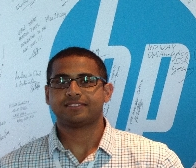
\includegraphics[width=.34\textwidth]{sai}
%
%            Sai Rahul Chalamalasetti
%
%            \textit{sairahul.chalamalasetti@hpe.com}
%        \end{center}
%
%        \column{0.5\textwidth}
%        \begin{center}
%            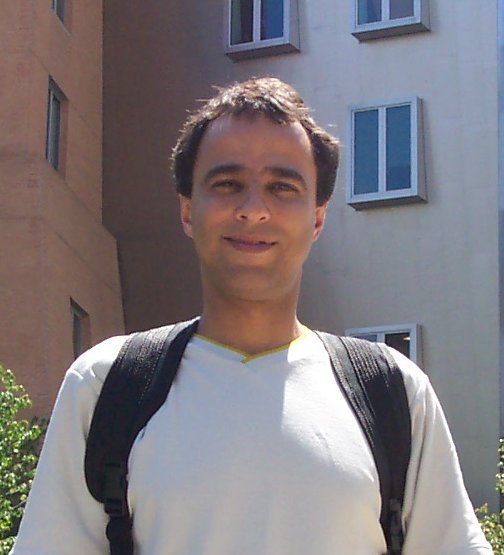
\includegraphics[width=.3\textwidth]{alfredo}
%
%            Alfredo Goldman
%
%            \textit{gold@ime.usp.br}
%        \end{center}
%
%        \begin{center}
%            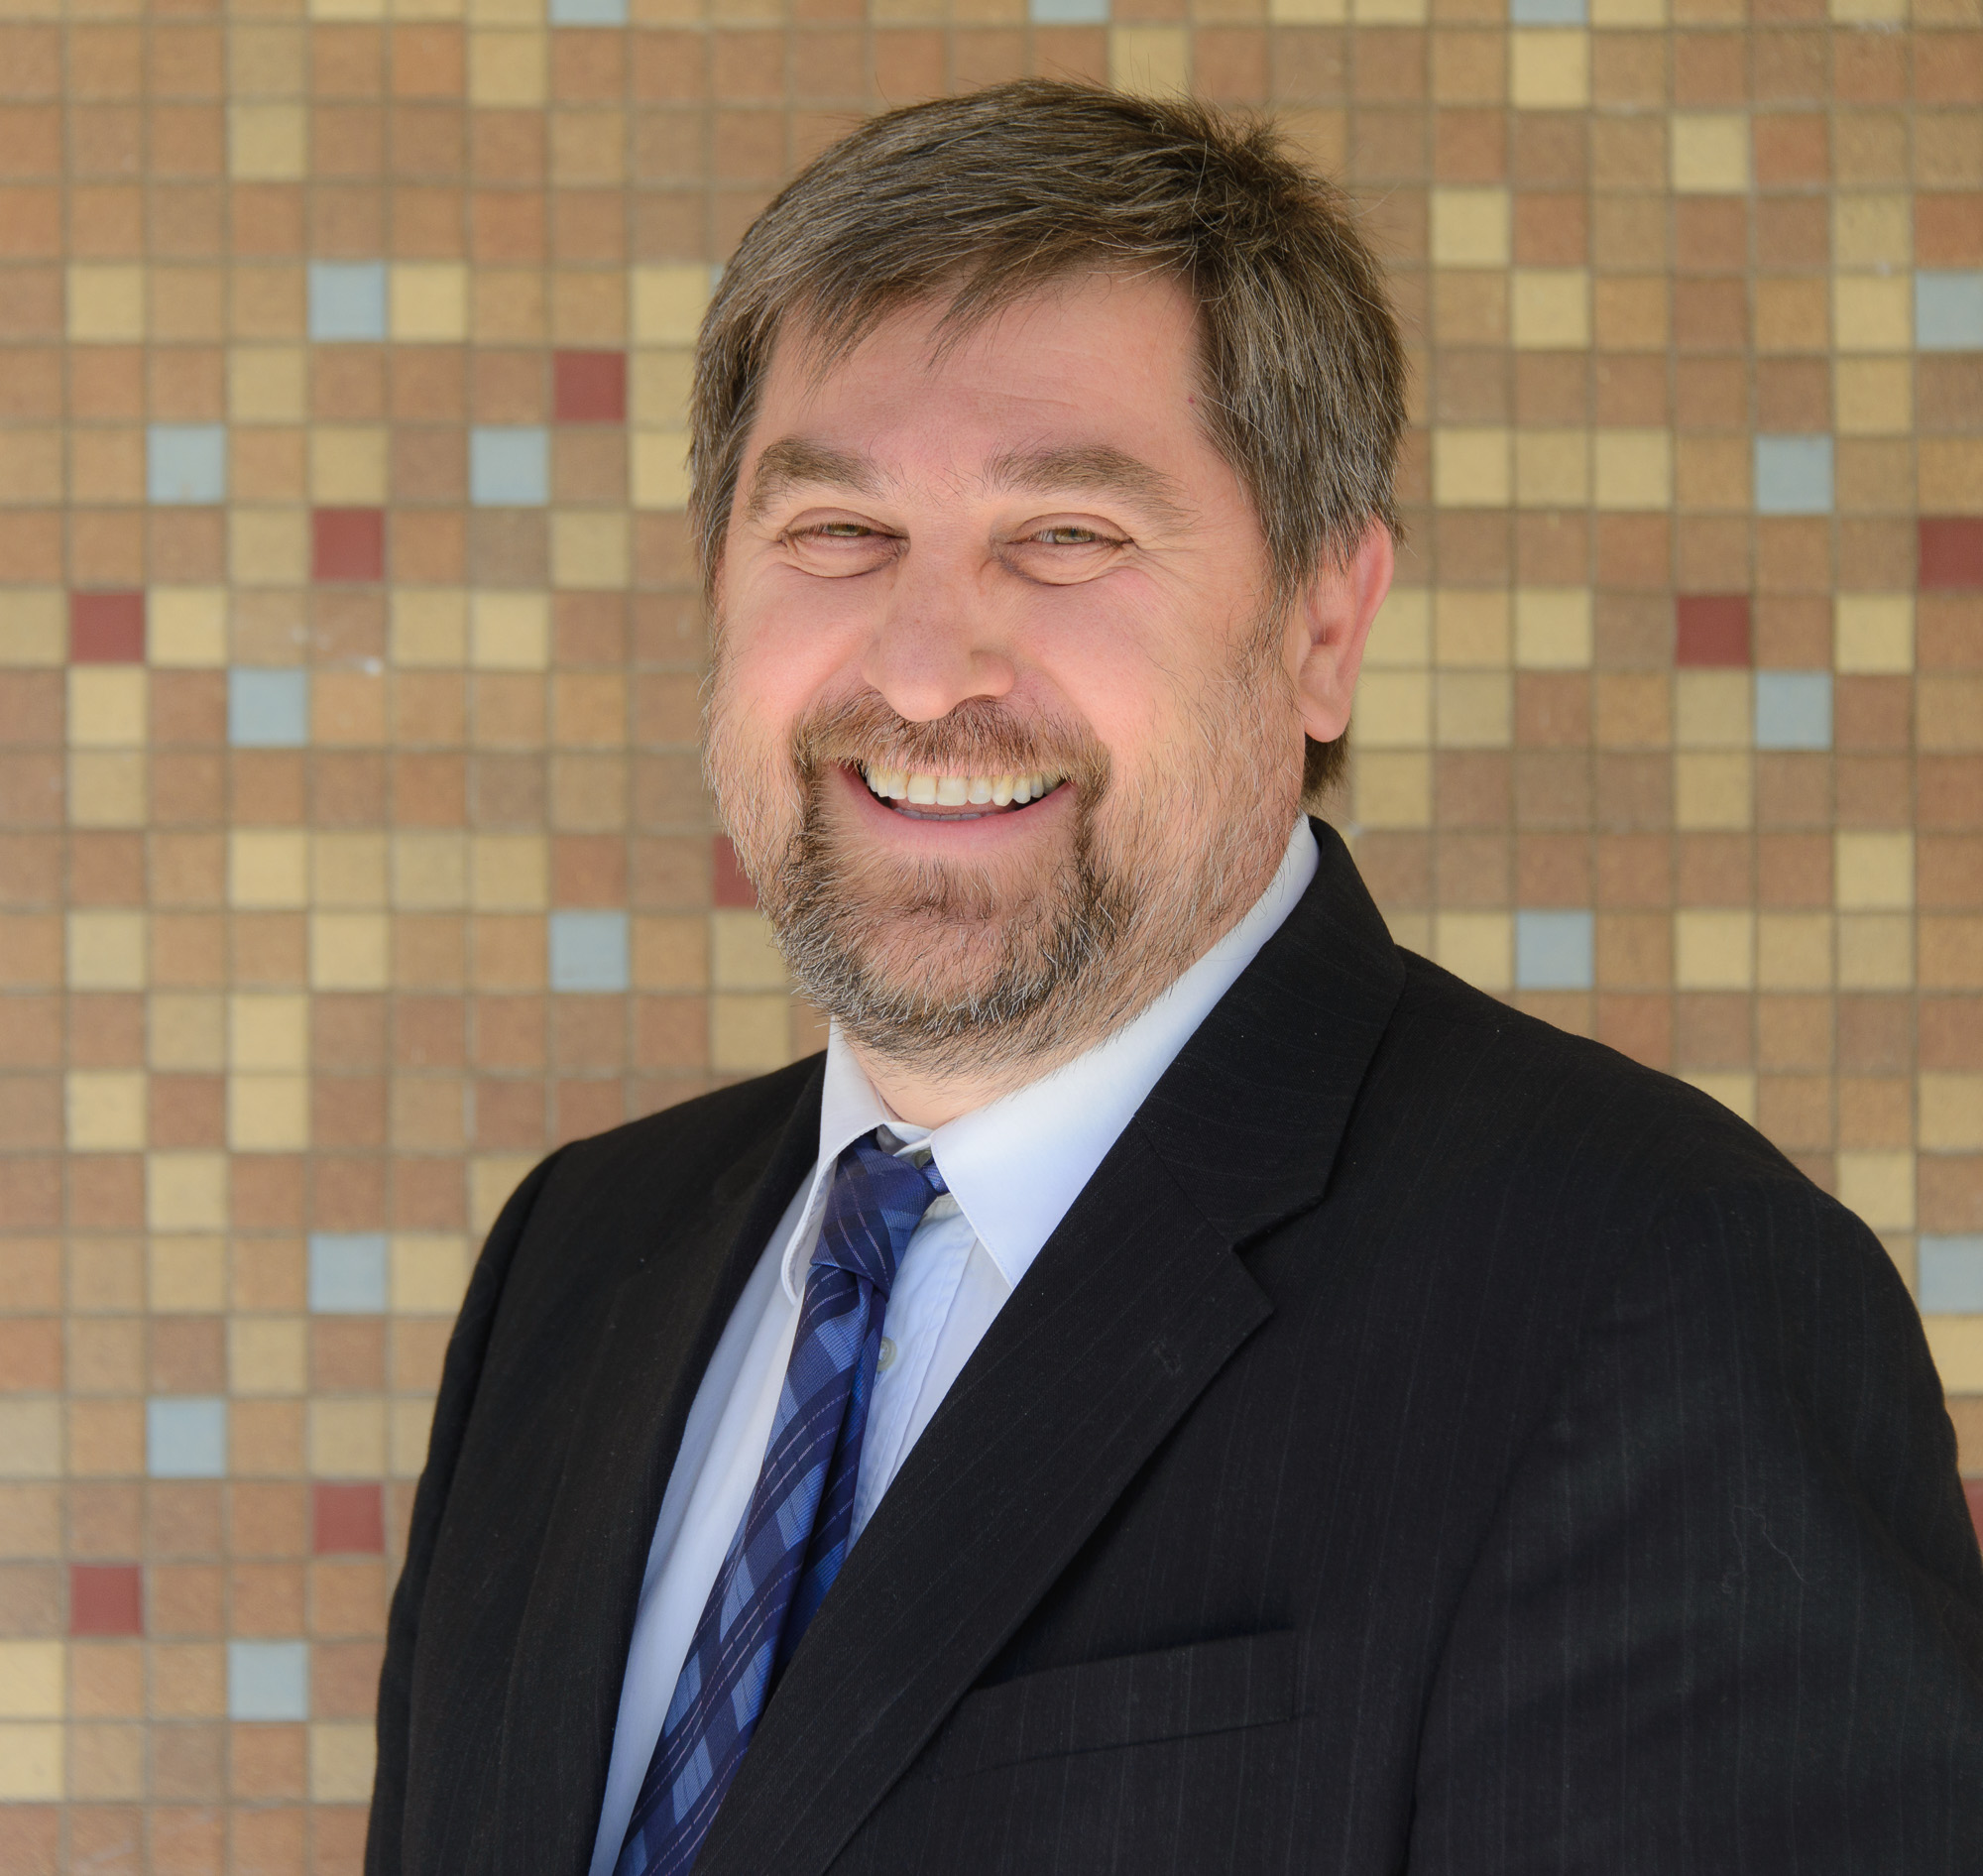
\includegraphics[width=.32\textwidth]{dejan}
%
%            Dejan Milojicic
%
%            \textit{dejan.milojicic@hpe.com}
%        \end{center}
%
%    \end{columns}
%\end{frame}

\begin{frame}
    \frametitle{Slides}
    \begin{center}
        
\includegraphics[width=.14\textwidth]{github}
    \end{center}
    The slides and all source code are hosted at \alert{GitHub}:

    \begin{itemize}
        \item \url{github.com/phrb/autotuning-workshop}
    \end{itemize}
\end{frame}

\subsection*{Outline}

\begin{frame}
    \frametitle{Outline}
    \setbeamertemplate{section in toc}[sections numbered]
    \tableofcontents[hideallsubsections]
\end{frame}

\section{Introduction to Autotuning}

\begin{frame}
    \frametitle{Autotuning: Optimization as a Search Problem}
    Casting program optimization as a \alert{search problem}:

    \begin{columns}[T,onlytextwidth]
        \column{0.5\textwidth}
        \alert{Search Spaces}:
        \begin{itemize}
            \item Algorithm Selections
            \item Program Configurations
            \item $\dots$
        \end{itemize}

        \column{0.5\textwidth}
        \alert{Search Objectives}:
        \begin{itemize}
            \item Minimize \alert{execution time}
            \item Maximize \alert{usage of resources}
            \item $\dots$
        \end{itemize}
    \end{columns}

    \vfill
\end{frame}

\begin{frame}
    \frametitle{Search Spaces \& Techniques}
    The \alert{search spaces} created by program optimization problems can be
    \alert{difficult to explore}

    \begin{center}
        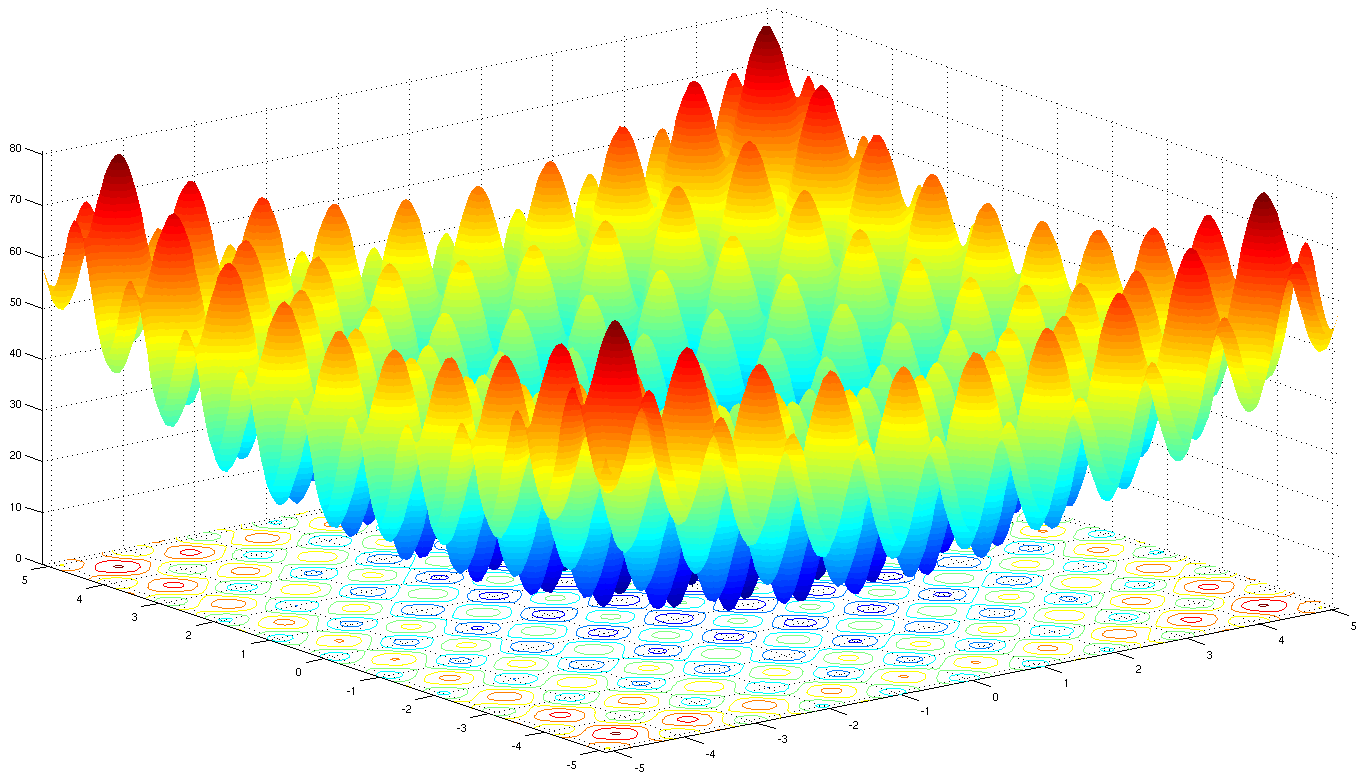
\includegraphics[width=.6\textwidth]{rastrigin}

        Rastrigin function, with \alert{global minimum} $f(0,0) = 0$
    \end{center}
\end{frame}

\begin{frame}
    \frametitle{Search Spaces \& Techniques}
    \begin{table}[]
        \centering
        \begin{tabular}{@{}lll@{}}
            \toprule
            System & Domain & Technique \\ \midrule
            ATLAS & Dense Linear Algebra & Exhaustive \\
            Insieme & Compiler & Genetic Algorithm \\
            SPIRAL & DSP Algorithms & Pareto Active Learning \\
            Active Harmony & Runtime & Nelder-Mead \\
            Periscope & HPC Applications & Various \\
            \alert{OpenTuner} & \alert{Domain-Agnostic} & \alert{Ensemble} \\ \bottomrule
        \end{tabular}
        \caption{Some autotuning systems, their domains and techniques}
    \end{table}

    \pause

    \begin{itemize}
        \item Different \alert{problem domains} generate different \alert{search spaces}
        \item \alert{No single solution} for all domains
        \item Search techniques can be composed: \alert{OpenTuner}
        \item Independent searches can be \alert{parallelized and distributed}
    \end{itemize}
\end{frame}

\begin{frame}
    \frametitle{Autotuning: Abstract Model}
    \begin{center}
        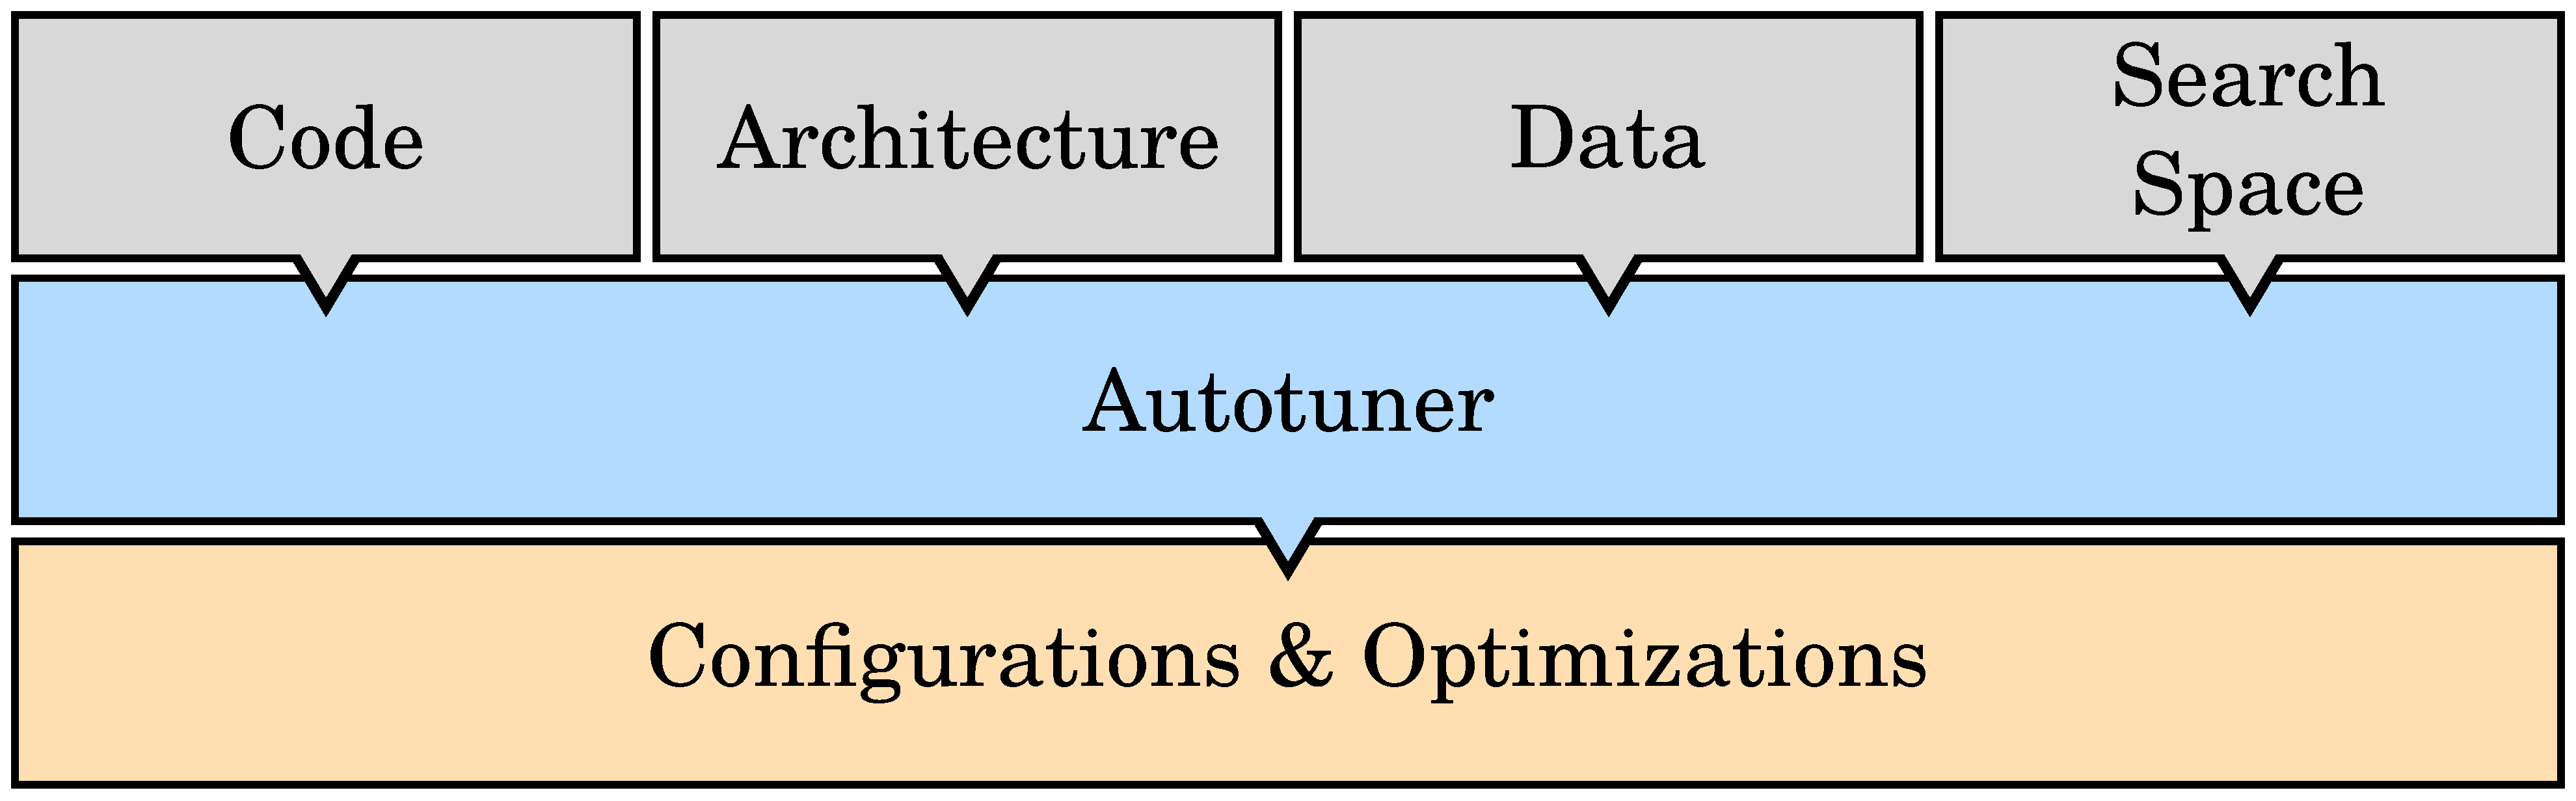
\includegraphics[width=.7\textwidth]{overview}
    \end{center}
\end{frame}

\section{Examples \& Results on Different Domains}

\begin{frame}
    \frametitle{NVIDIA CUDA Compiler: From CUDA C++ to Object Code}
    \begin{center}
        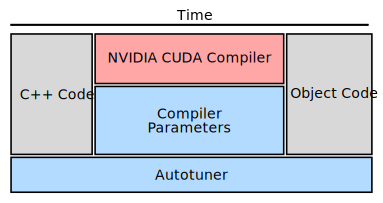
\includegraphics[width=.6\textwidth]{gpu-stack}
    \end{center}

    \begin{itemize}
        \item We tuned applications from the \alert{Rodinia Benchmark Suite}
        \item C++ $\rightarrow$ Object Code: takes \alert{seconds}
    \end{itemize}
\end{frame}

\begin{frame}
    \frametitle{Autotuning: GPUs}
    \begin{center}
        
\includegraphics[width=.7\textwidth]{overview_gpus}

        \vspace{.3cm}

        \alert{1h} of tuning $\rightarrow \; \approx \alert{10^3}$ \alert{iterations}
    \end{center}
\end{frame}


\begin{frame}
    \frametitle{Results}
    \alert{Most significative speedups} for \alert{Rodinia applications}
    and \alert{matrix multiplication optimizations}, after \alert{1.5h of tuning}:

    \begin{center}
        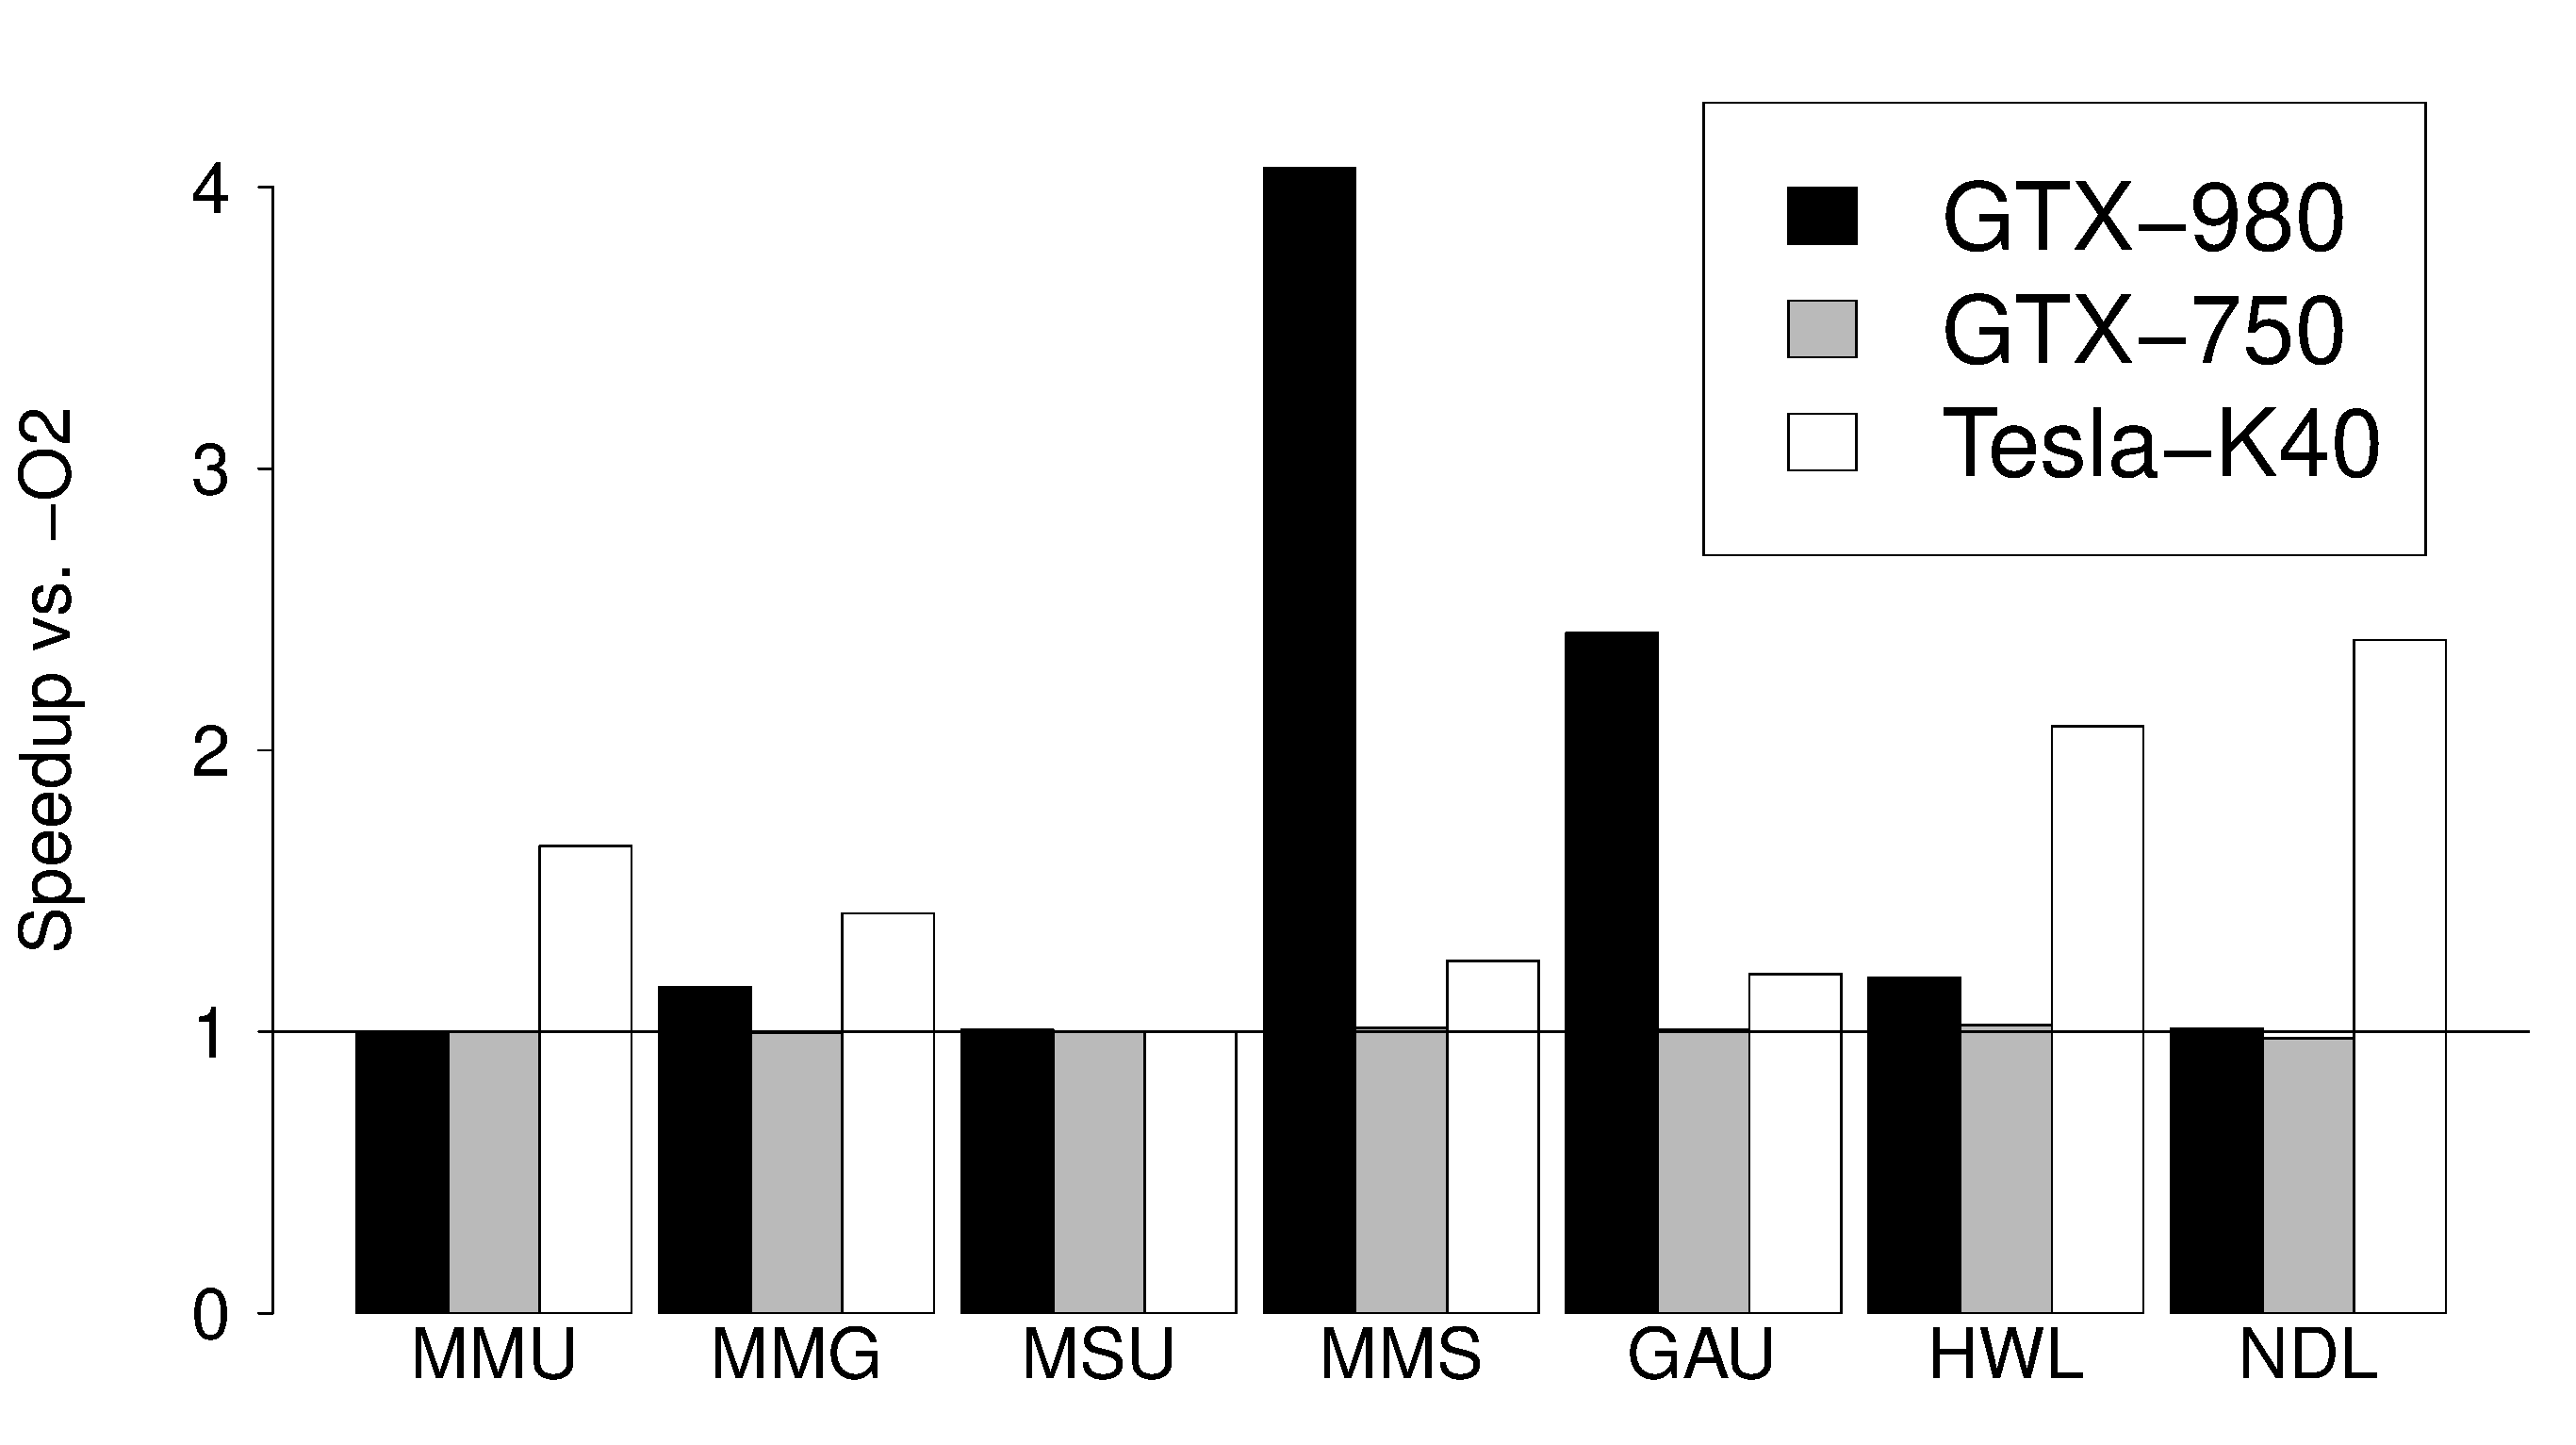
\includegraphics[width=.6\textwidth]{GPU-tuning-summary}
    \end{center}

    We \alert{found no globally good parameter selections} for specific GPUs or applications
\end{frame}

\begin{frame}
    \frametitle{High-Level Synthesis for FPGAs: From C to Hardware}
    \begin{center}
        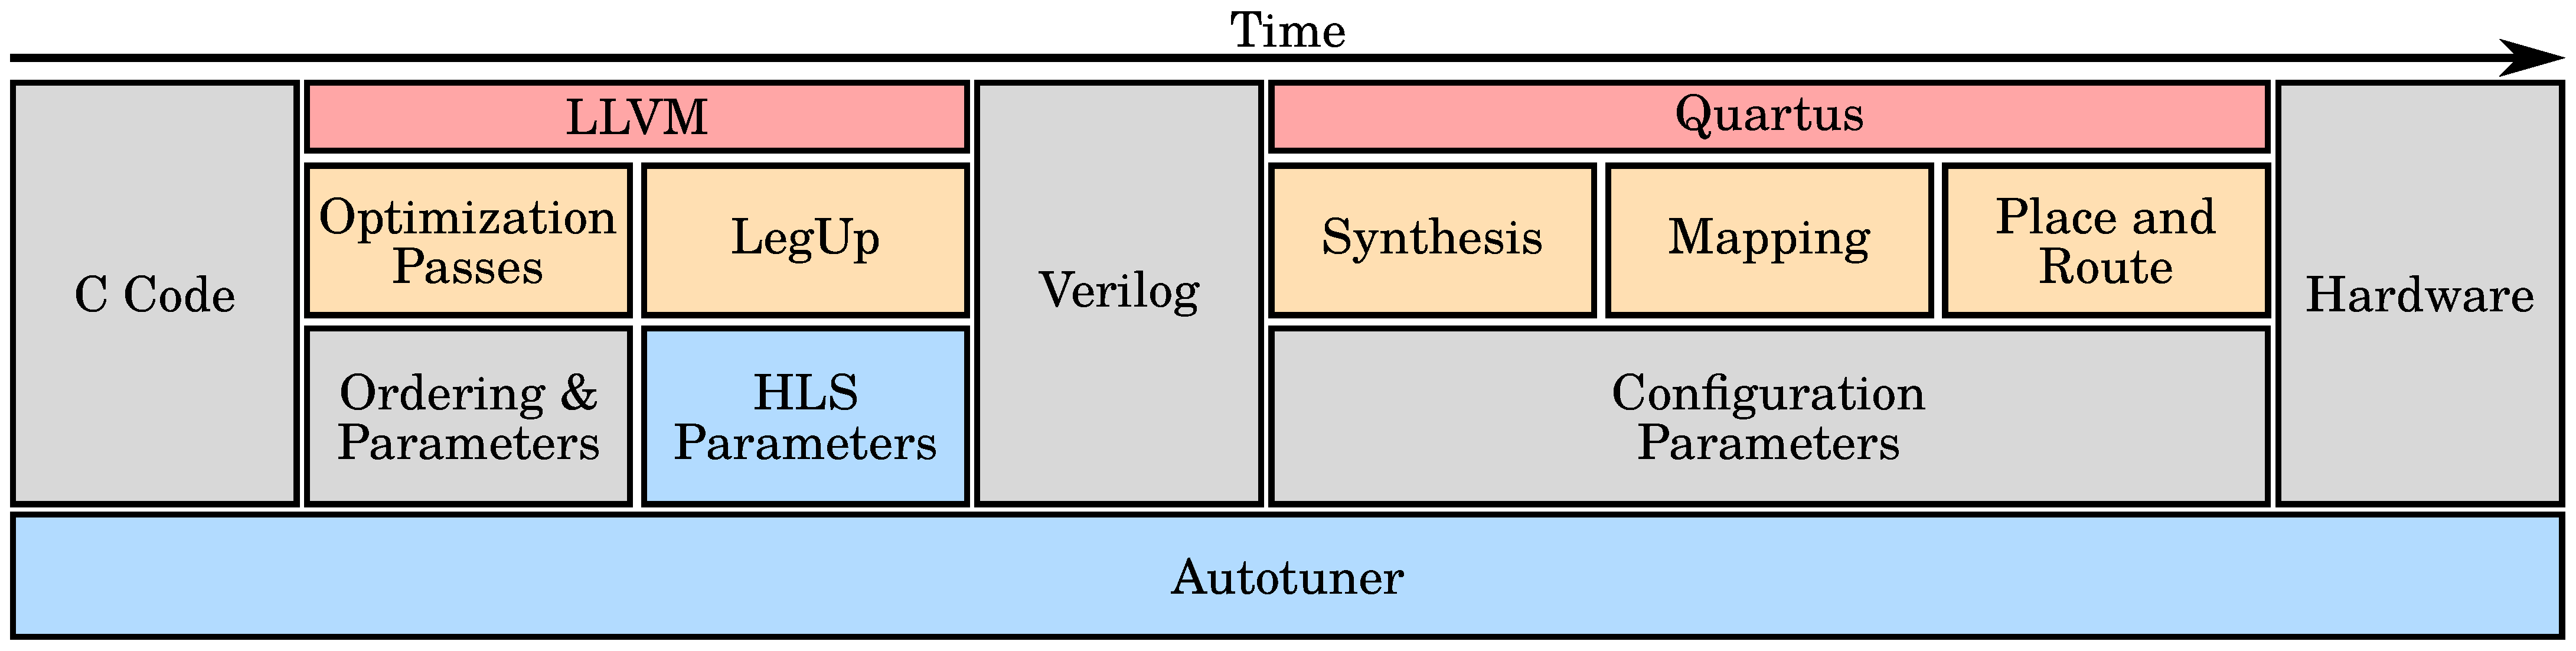
\includegraphics[width=1\textwidth]{fpga-stack}
    \end{center}

    \begin{itemize}
        \item We tuned applications from the \alert{CHStone Benchmark Suite}
        \item C $\rightarrow$ Verilog: takes \alert{seconds}
        \item Verilog $\rightarrow$ Hardware: takes \alert{minutes}, \alert{hours}
    \end{itemize}
\end{frame}

\begin{frame}
    \frametitle{Autotuning LegUp Parameters for CHStone}
    \begin{center}
        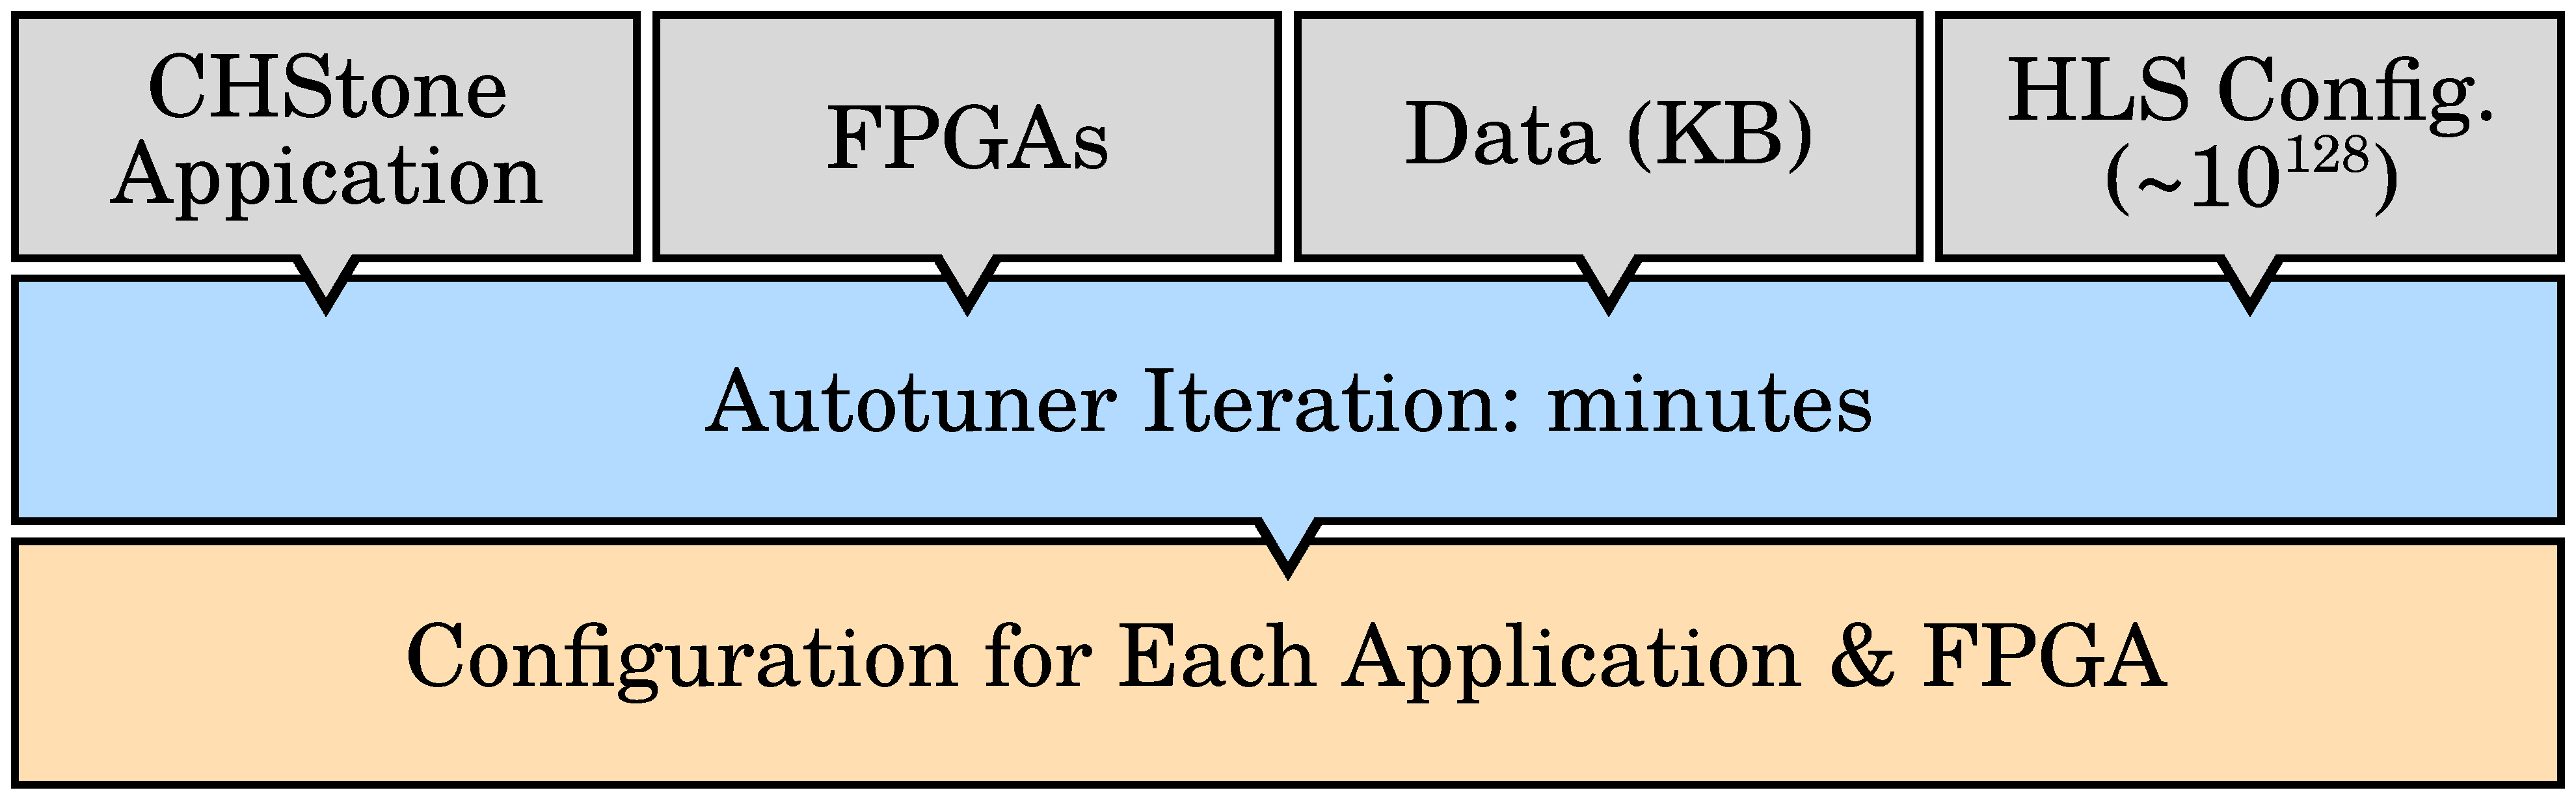
\includegraphics[width=.7\textwidth]{overview_fpgas_small}

        \vspace{.3cm}

         \alert{1h} of tuning $\rightarrow \; \approx \alert{10}$ \alert{iterations}
    \end{center}
\end{frame}

%\begin{frame}
%    \frametitle{Autotuning LegUp Parameters for CHStone}
%    \alert{Search Space}:
%    \begin{itemize}
%        \item \alert{LegUp constraints} that impact \alert{Verilog generation}
%        \item Read from a \alert{configuration file}
%    \end{itemize}
%
%    Examples:
%    \begin{itemize}
%        \item \texttt{set\_accelerator\_function}
%        \item \texttt{ENABLE\_PATTERN\_SHARING}
%    \end{itemize}
%
%    \begin{center}
%        \tiny{Source: \url{legup.eecg.utoronto.ca/docs/4.0/constraintsmanual.html\#constraints} [Accessed on 15/09/16]}
%    \end{center}
%\end{frame}

\begin{frame}
    \frametitle{Autotuning LegUp Parameters for CHStone}
    Computing the \alert{fitness function}:

    \begin{align*} \label{eq:wnsm}
        \mathlarger{f(M, W)} = \frac{\mathlarger{\mathlarger{\mathlarger{\sum}}}\limits_{\substack{m_i \in M \\ w_i \in W}}{w_i\left(\dfrac{m_i}{m_{i}^{0}}\right)}}{\mathlarger{\mathlarger{\mathlarger{\sum}}}\limits_{w_i \in W}{w_i}}
    \end{align*}

    \begin{itemize}
        \item $M$: the set of \alert{metrics}
        \item $W$: the set of \alert{weights for each metric}
        \item $m_{i}^{0}$: \alert{initial measured value} for each metric
        \item $f(M,W)$: \alert{cost} or \alert{fitness function}, defined as
    \end{itemize}
\end{frame}

\begin{frame}[fragile]
    \frametitle{Next Steps: Meaningful Metric Weights}

    Relative weights in \alert{different scenarios}:

    \begin{table}[htpb]
    \centering
    \begin{tabular}{@{}lcccc@{}}
        \toprule
        Metric & \textit{Area} & \textit{Perf. \& Lat} & \textit{Performance} & \textit{Balanced} \\ \midrule
        \textit{LUT} & \cellcolor[HTML]{9B94B6} High & \cellcolor[HTML]{DD9583} Low & \cellcolor[HTML]{DD9583} Low & \cellcolor[HTML]{E3DBB3} Medium \\
        \textit{Registers} & \cellcolor[HTML]{9B94B6} High & \cellcolor[HTML]{9B94B6} High & \cellcolor[HTML]{E3DBB3} Medium & \cellcolor[HTML]{E3DBB3} Medium \\
        \textit{BRAMs} & \cellcolor[HTML]{9B94B6} High & \cellcolor[HTML]{DD9583} Low & \cellcolor[HTML]{DD9583} Low & \cellcolor[HTML]{E3DBB3} Medium \\
        \textit{DSPs} & \cellcolor[HTML]{9B94B6} High & \cellcolor[HTML]{DD9583} Low & \cellcolor[HTML]{DD9583} Low & \cellcolor[HTML]{E3DBB3} Medium \\
        \textit{FMax} & \cellcolor[HTML]{DD9583} Low & \cellcolor[HTML]{9B94B6} High & \cellcolor[HTML]{9B94B6} High & \cellcolor[HTML]{E3DBB3} Medium \\
        \textit{Cycles} & \cellcolor[HTML]{DD9583} Low & \cellcolor[HTML]{9B94B6} High & \cellcolor[HTML]{DD9583} Low & \cellcolor[HTML]{E3DBB3} Medium \\ \bottomrule
    \end{tabular}
    \caption{Weights for Optimization Scenarios (\textit{High} $= 8$, \textit{Medium} $= 4$, \textit{Low} $= 2$)}
    \label{tab:scenarios}
    \end{table}
\end{frame}

\begin{frame}
    \frametitle{Results in Different Optimization Scenarios}
    Decreases for the \alert{Weighted Normalized Sum} of
    hardware metrics in \alert{4 optimization scenarios}, mean of \alert{10
    tuning runs} of \alert{1.5h each}, for the \alert{StratixV DE5} FPGA:

    \begin{center}
        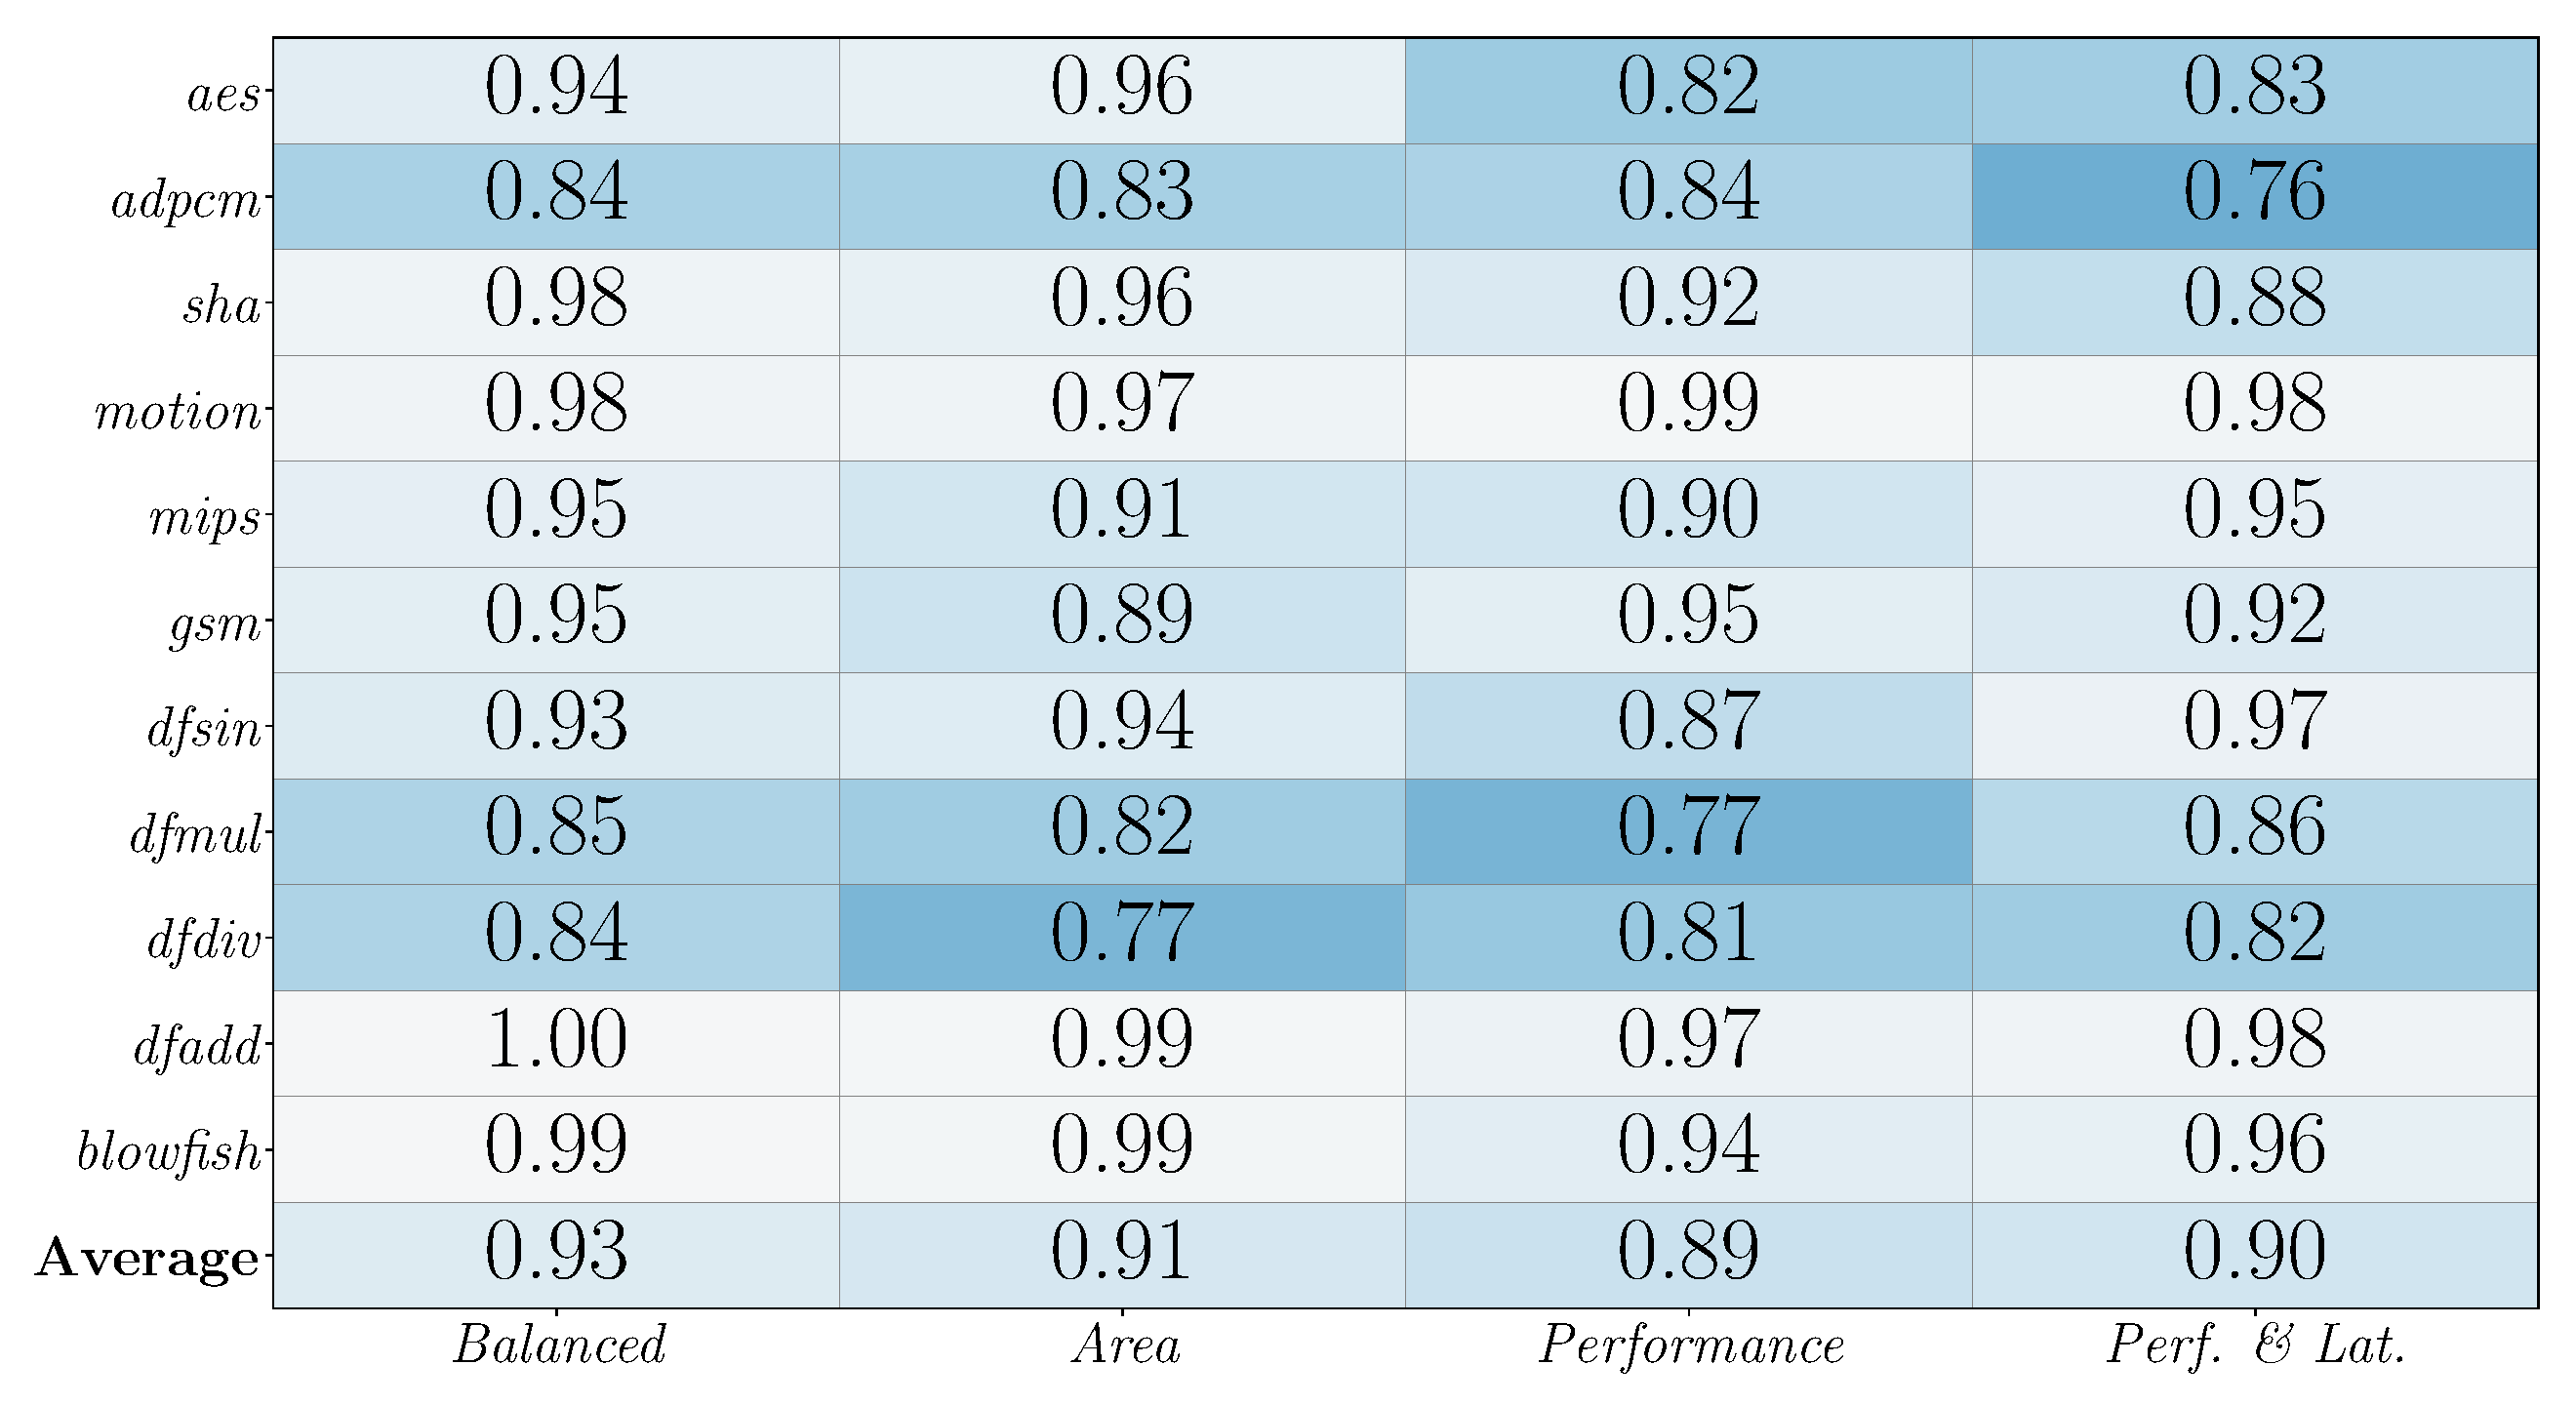
\includegraphics[width=0.8\textwidth]{heatmap_wns_comparison}
    \end{center}
\end{frame}

\begin{frame}
    \frametitle{Results in the Performance Scenario}
    Decreases for \alert{all hardware metrics}
    in the \alert{Performance} scenario:

    \begin{center}
        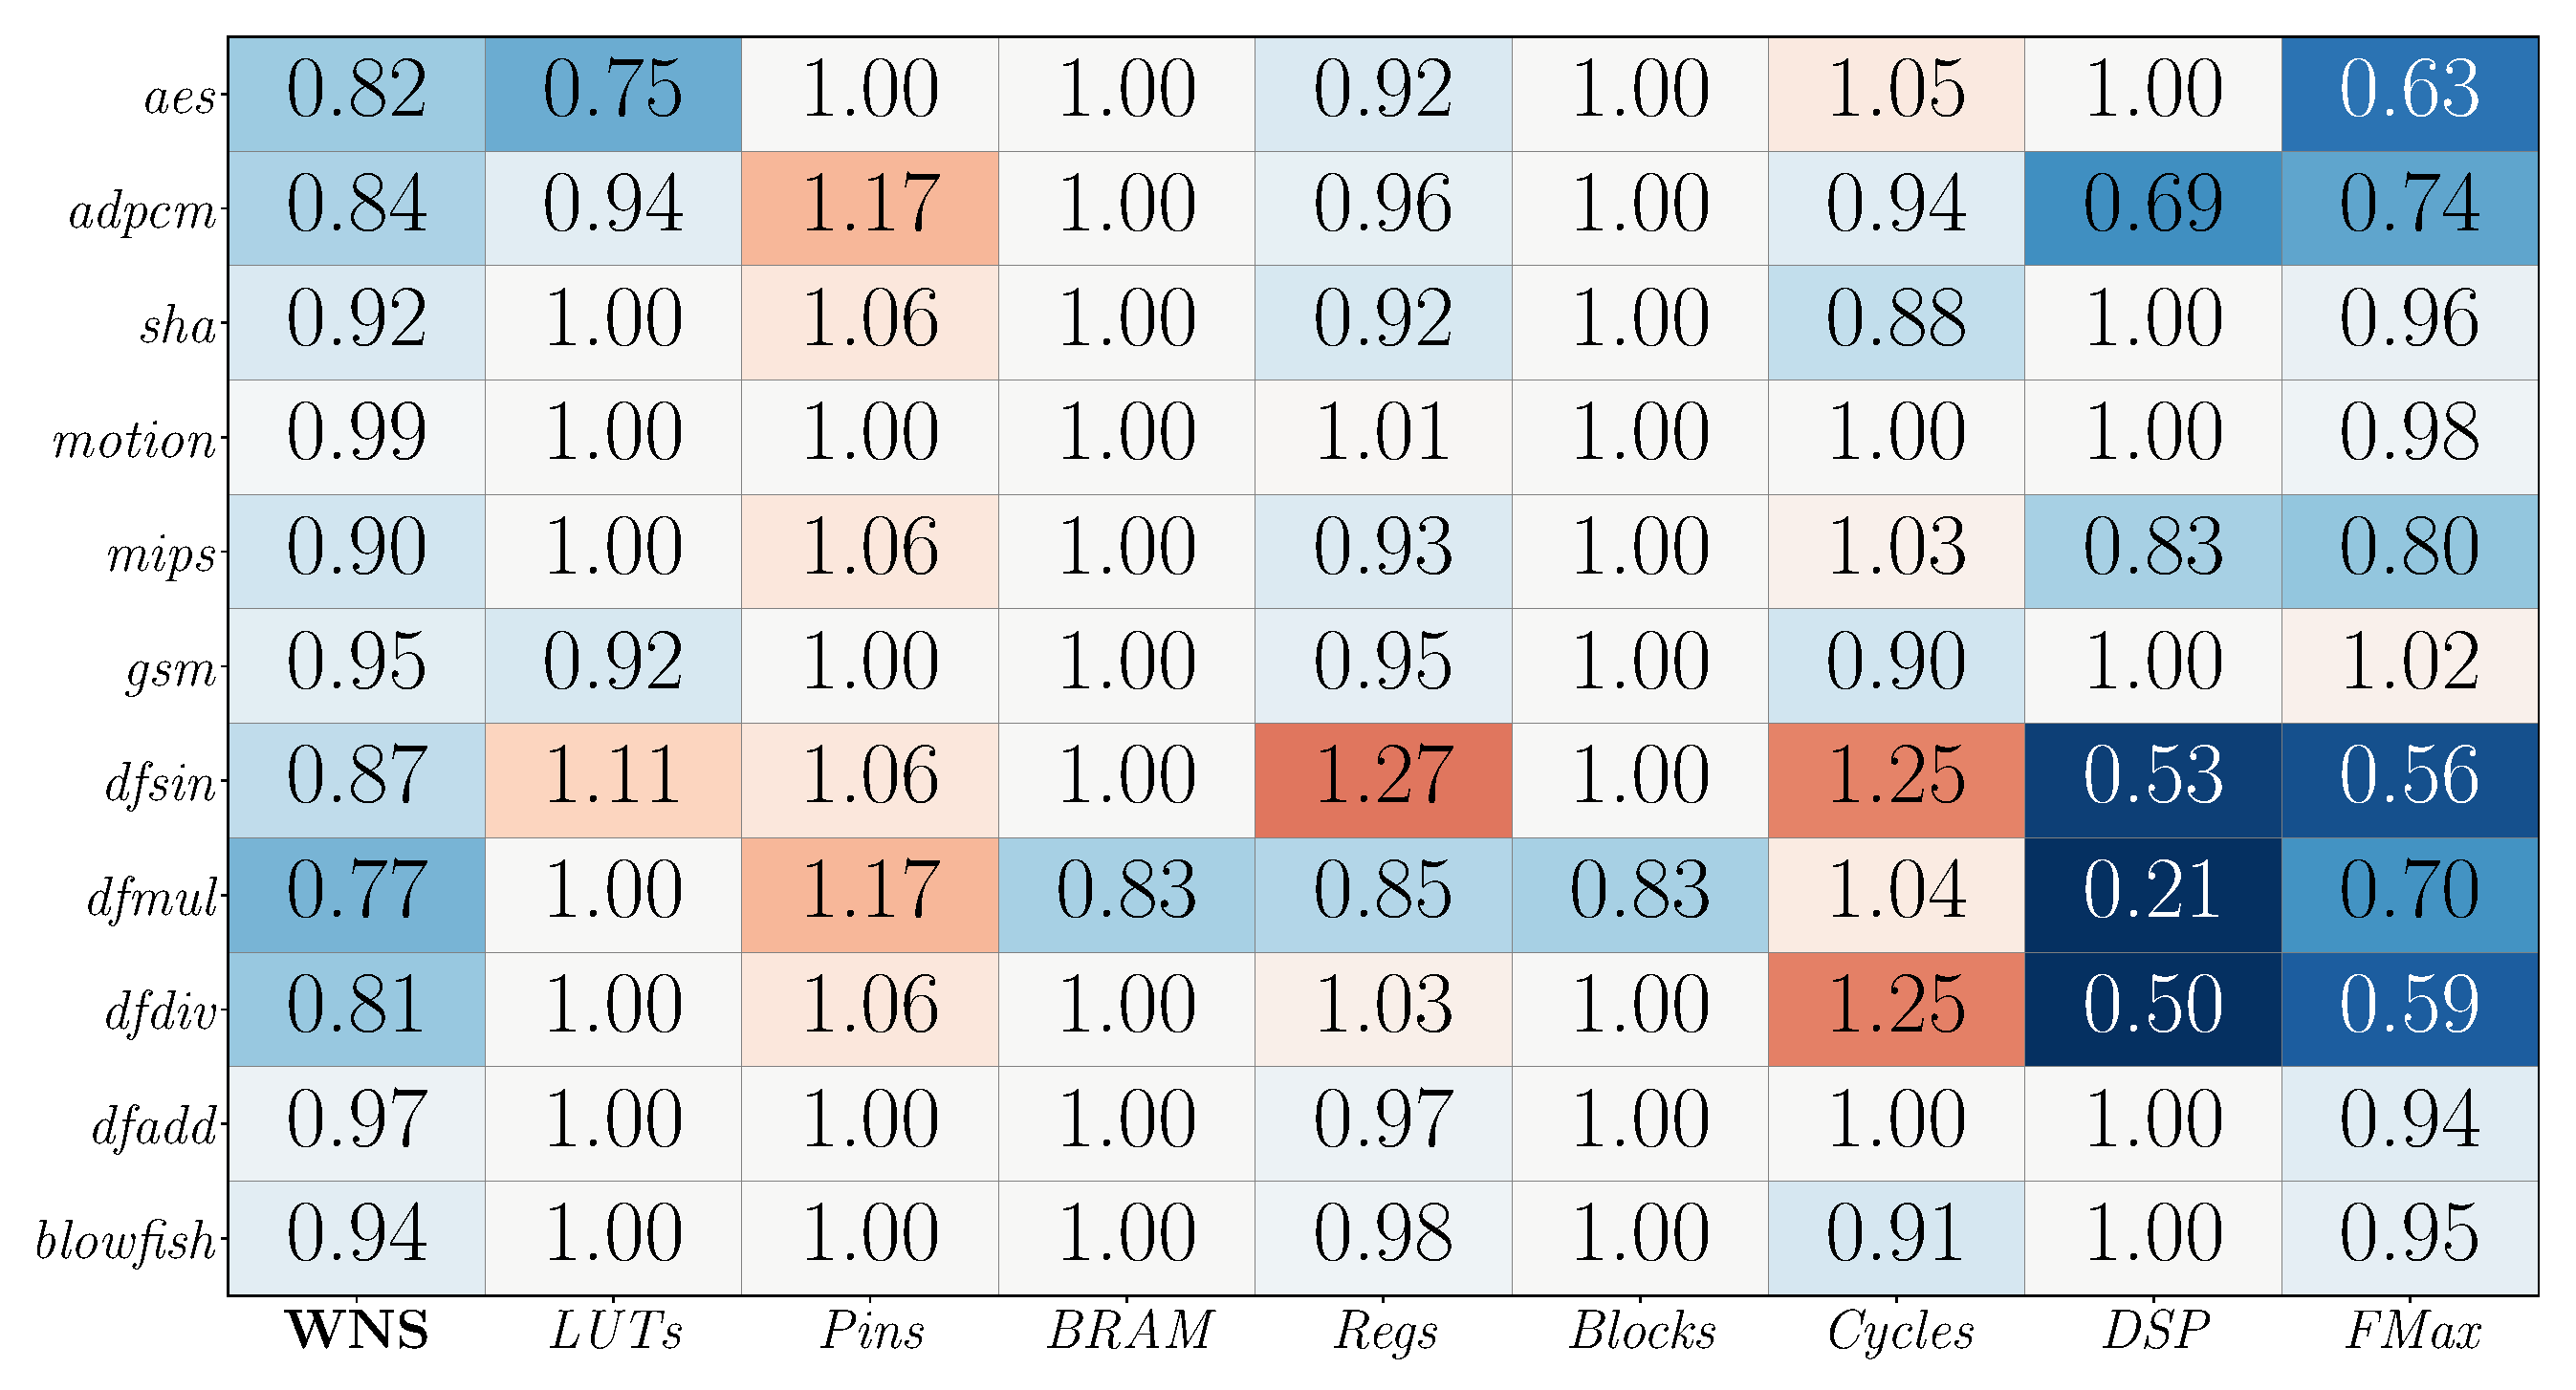
\includegraphics[width=0.8\textwidth]{heatmap_default_stratixV_perf}
    \end{center}
\end{frame}

\begin{frame}
    \frametitle{Current Challenges: Expensive-to-Evaluate Functions}
    \begin{center}
        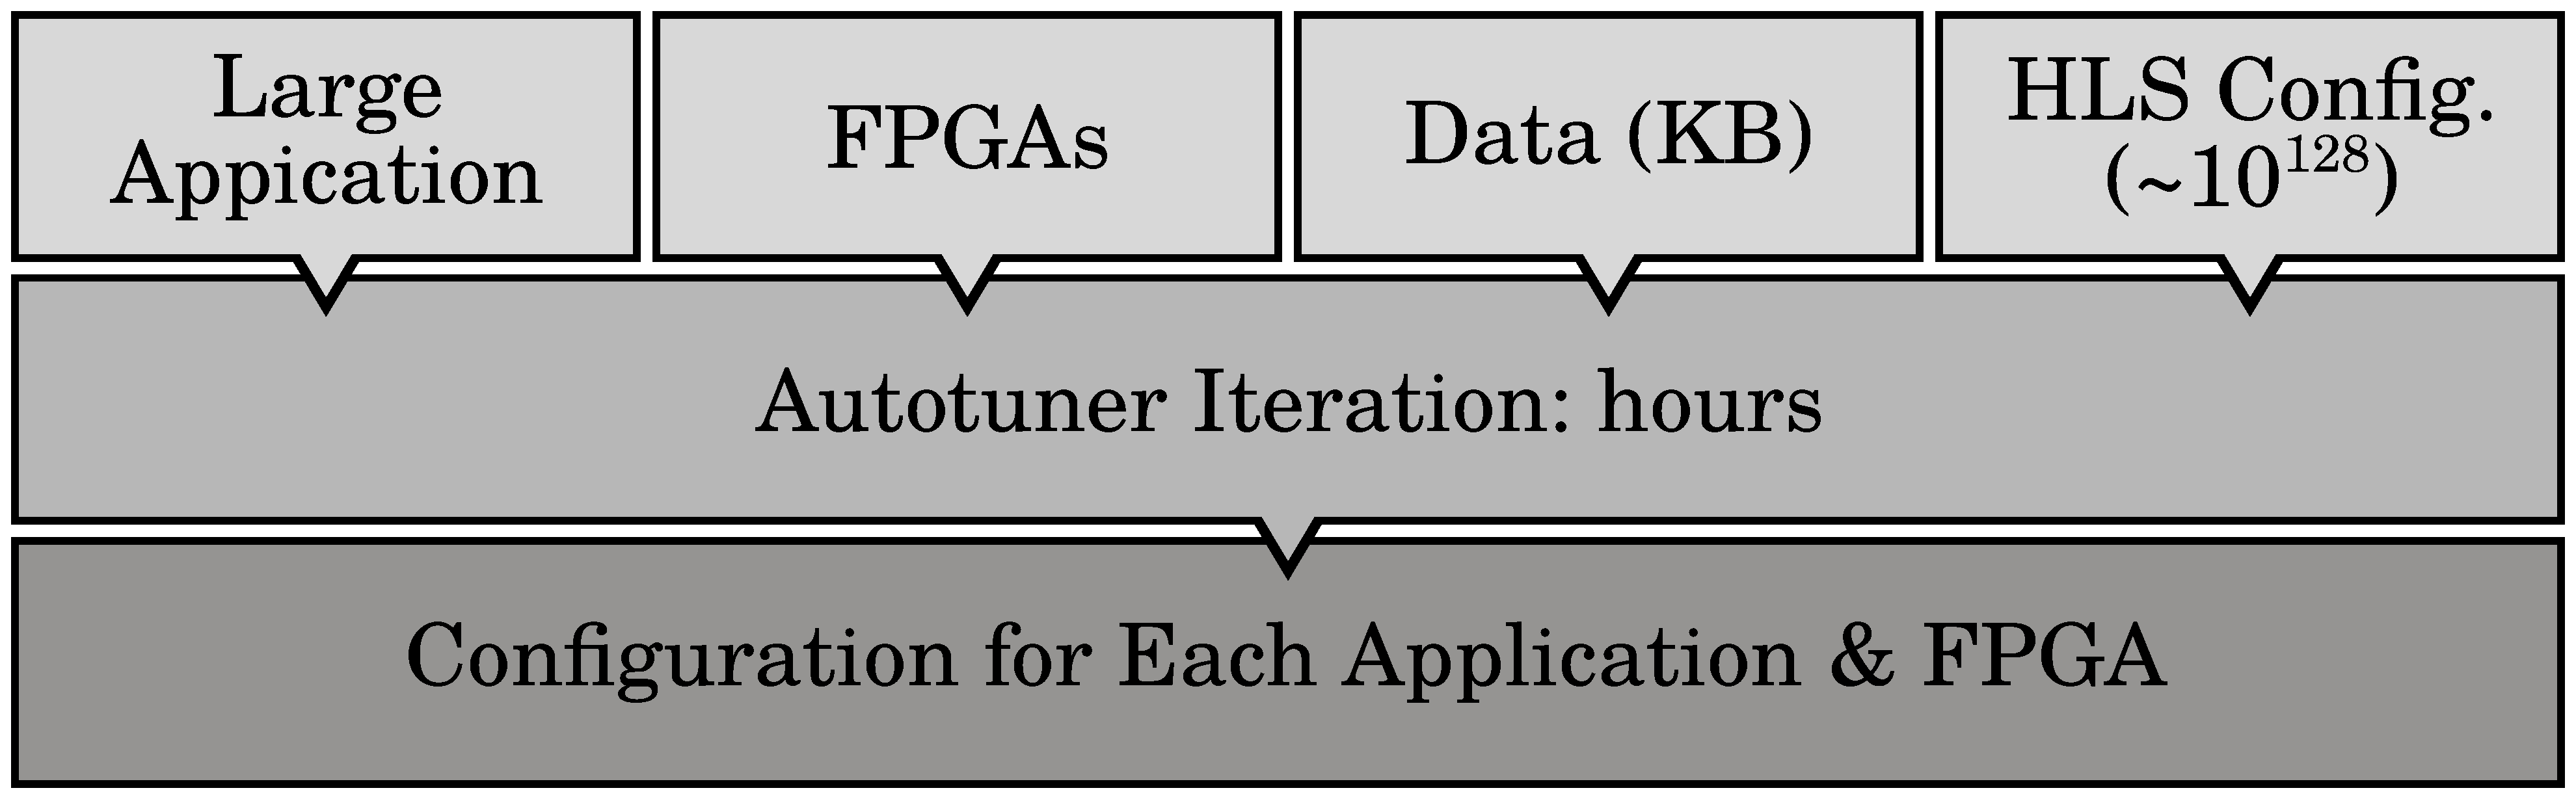
\includegraphics[width=.7\textwidth]{overview_fpgas_big}
    \end{center}

    \vspace{.3cm}

    \begin{itemize}
        \item \alert{1h} of tuning $\rightarrow \; \approx \alert{1}$ \alert{iteration}
        \item Iterations now \alert{take too long}
    \end{itemize}
\end{frame}

\begin{frame}
    \frametitle{Current Challenges: Autotuning the HPE Dot Product Engine}
    The \alert{Dot Product Engine} (\alert{DPE}):

    \begin{itemize}
        \item An experimental architecture from \alert{Hewlett-Packard Enterprise}
        \item Specialized in \alert{Convolutional Neural Networks}
        \item Used for the \alert{inference step} in Machine Learning
    \end{itemize}
\end{frame}

\begin{frame}
    \frametitle{Current Challenges: Autotuning the HPE Dot Product Engine}
    \vspace{.4cm}

    \begin{center}
        \includegraphics[width=.6\textwidth]{dpe-arch}
    \end{center}
\end{frame}

\begin{frame}
    \frametitle{Current Challenges: Autotuning the HPE Dot Product Engine}
    \alert{Hardware Design} and \alert{Software} autotuning opportunities:

    \begin{center}
        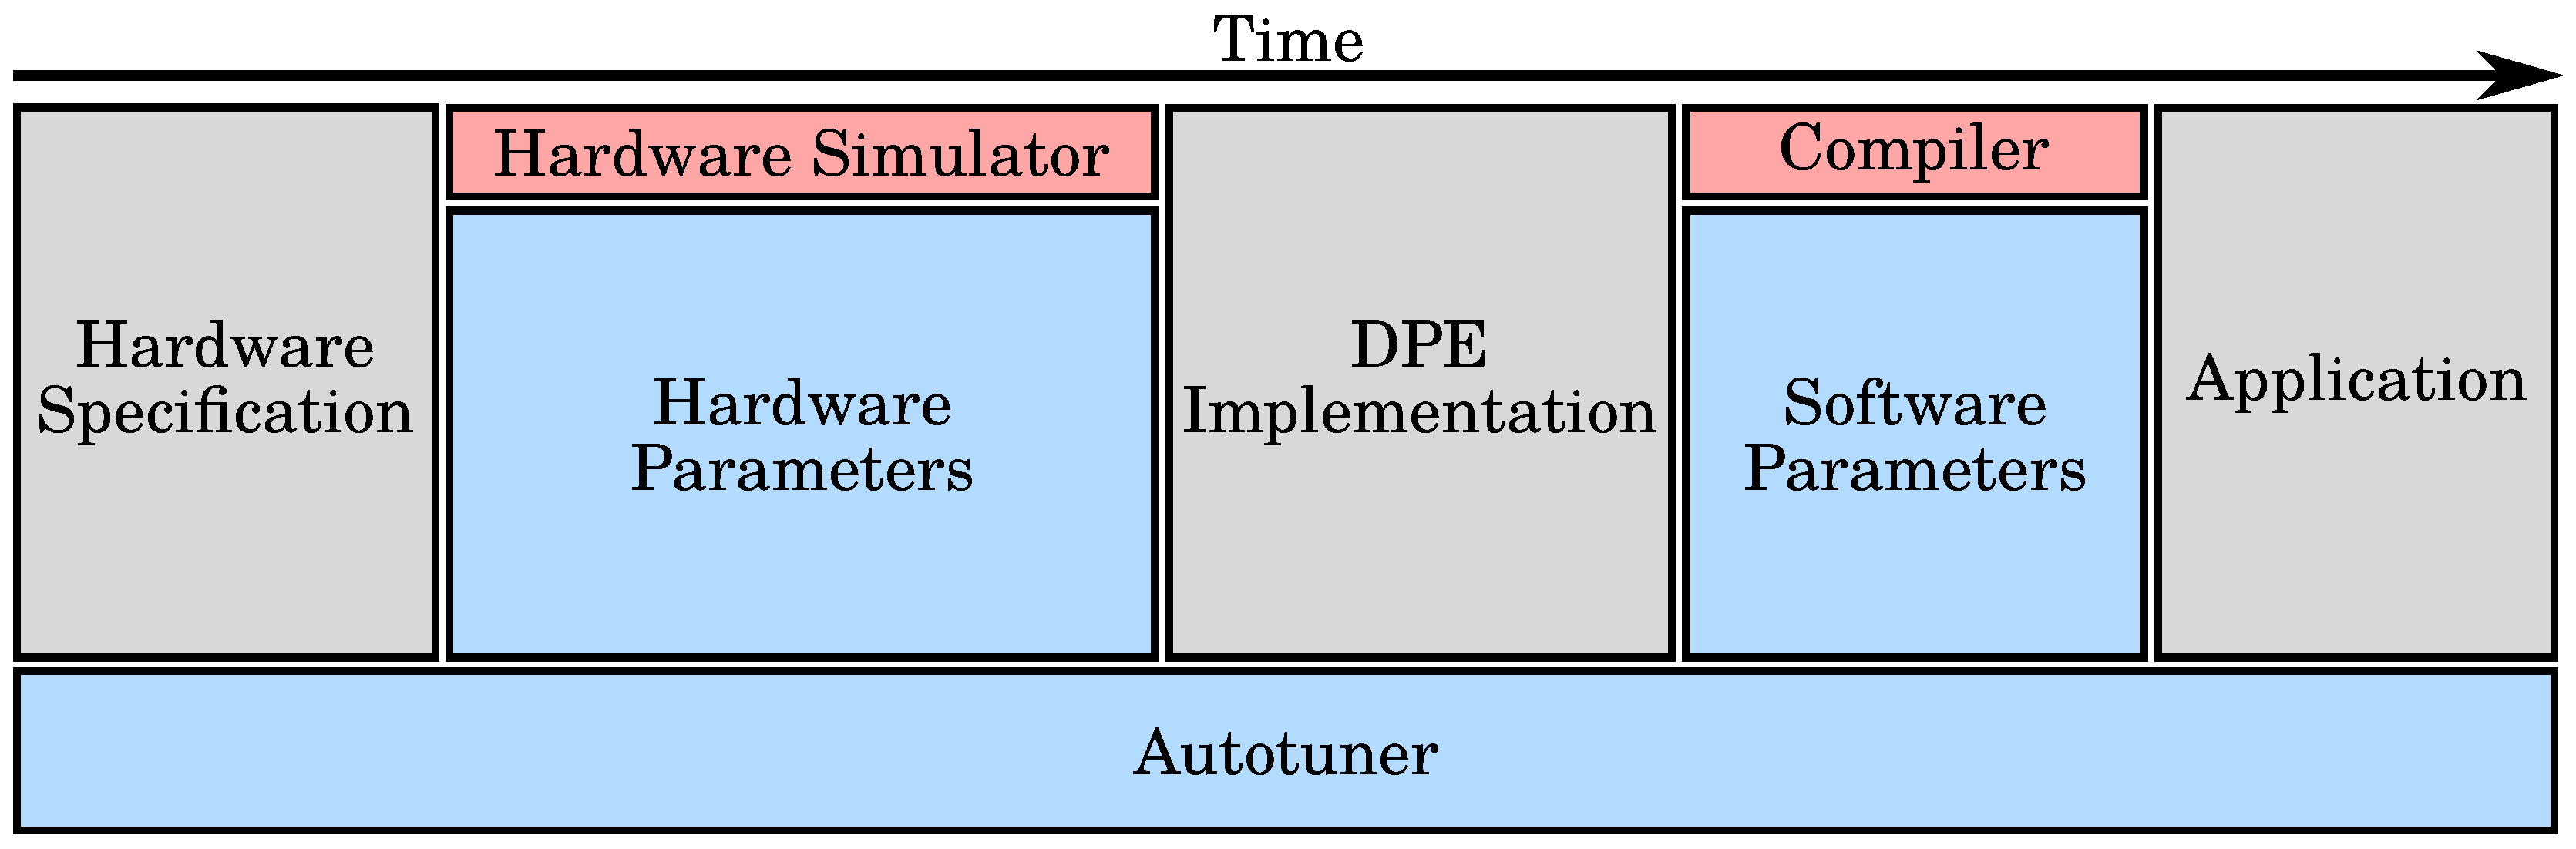
\includegraphics[width=.7\textwidth]{dpe-stack}
    \end{center}
\end{frame}

\begin{frame}
    \frametitle{Current Challenges: Autotuning the HPE Dot Product Engine}
    Autotuning \alert{hardware and software} in the context of the \alert{DPE}:

    \begin{columns}[T,onlytextwidth]
        \column{0.5\textwidth}
        \alert{Hardware search space}:
        \begin{itemize}
            \item ADC Configuration
            \item Communication between tiles
            \item Number of crossbars, IMAs in tiles
            \item Size of DPE, routing tables, eDRAM buffers
            \item $\dots$
        \end{itemize}

        \alert{DPE metrics}:
        \begin{itemize}
            \item Usability
            \item Bandwidth, Latency, Throughput
            \item Computation and Power Efficiency
            \item $\dots$
        \end{itemize}

        \column{0.5\textwidth}
        \alert{Software search space}:
        \begin{itemize}
            \item ADC usage
            \item Tile usage
            \item Mapping to memristor arrays, layers, routing tables
            \item $\dots$
        \end{itemize}

        \alert{Measurement using models}:
        \begin{itemize}
            \item Area and power overhead for components
            \item Cycle accurate simulations for accessing eDRAM, communicating tiles
            \item $\dots$
        \end{itemize}
    \end{columns}

    \vfill
\end{frame}

\section{An Autotuning Library in the Julia Language}

\begin{frame}
    \frametitle{An Autotuning Library in the Julia Language}
    \begin{center}
        
\includegraphics[width=.25\textwidth]{stochasticsearch_logo}
    \end{center}

    We are developing an autotuning library:
    \begin{itemize}
        \item In the \alert{Julia} language
        \item \alert{Domain-Agnostic}
        \item \alert{Parallel and distributed autotuning}
        \item \url{github.com/phrb/StochasticSearch.jl}
    \end{itemize}
\end{frame}

\begin{frame}
    \frametitle{StochasticSearch: Search Techniques}
    Multiple \alert{simultaneous search techniques} share a search space, but
    not results:

    \vspace{.3cm}

    \begin{columns}[T,onlytextwidth]
        \column{0.5\textwidth}
        \alert{Implemented} techniques:
        \begin{itemize}
            \item Simulated Annealing
            \item Iterated Local Search
            \item Randomized First Improvement
            \item Iterative First Improvement
            \item Iterative Probabilistic Improvement
            \item Iterative Greedy Construction
        \end{itemize}

        \pause

        \column{0.5\textwidth}
        \alert{Future} techniques:
        \begin{itemize}
            \item Best Improvement
            \item Iterative Best Improvement
            \item Randomized Best Improvement
            \item Dynamic Local Search
            \item Tabu Search
            \item Ant Colony Optimization
            \item $\dots$
        \end{itemize}
    \end{columns}
\end{frame}

\begin{frame}
    \frametitle{Why use the Julia Language?}
    \begin{center}
        
\includegraphics[width=.2\columnwidth]{julia_logo}
    \end{center}

    Why the \alert{Julia Language}?

    \begin{itemize}
        \item \alert{High-Level abstractions}
        \item \alert{Simple interface} for parallel and distributed programming
        \item \alert{Better performance} than Python, Matlab, R, $\dots$
    \end{itemize}
\end{frame}

\begin{frame}
    \frametitle{Parallel and Distributed Programming in Julia}
    Parallel and Distributed programming:

    \begin{itemize}
        \item \alert{Process-based} parallelism
        \item \alert{Communication} between processes uses \alert{channels}
        \item \alert{Serialize/Deserialize} complex data types
            \pause
        \item Works on \alert{many-core and clouds} using an MPI-like \alert{machinefile}
        \item \alert{No shared memory} yet, with \alert{experimental native threading}
    \end{itemize}

    \pause

    Simple interface:

    \begin{itemize}
        \item \alert{Remote execution} on a \alert{new process}: \texttt{remotecall($\cdot$)} and \texttt{@spawn}
        \item \alert{Channels}: \texttt{put!($\cdot$)} and \texttt{take!($\cdot$)}
    \end{itemize}
\end{frame}

\begin{frame}
    \frametitle{StochasticSearch Example: The Rosenbrock Function}
    Let's create a \alert{Tuning Run} using \alert{StochasticSearch}:
    \begin{columns}[T,onlytextwidth]
        \column{0.5\textwidth}
        \vspace{1cm}

        The Rosenbrock function:
        \begin{itemize}
            \item \alert{Global minimum} $f(1,1) = 0$
            \item Many \alert{local minima}
        \end{itemize}

        \vspace{.5cm}

        Components:
        \begin{itemize}
            \item \alert{Parameters}
            \item \alert{Configurations}
            \item \alert{Cost Function}
        \end{itemize}

        \column{0.5\textwidth}
        \begin{center}
            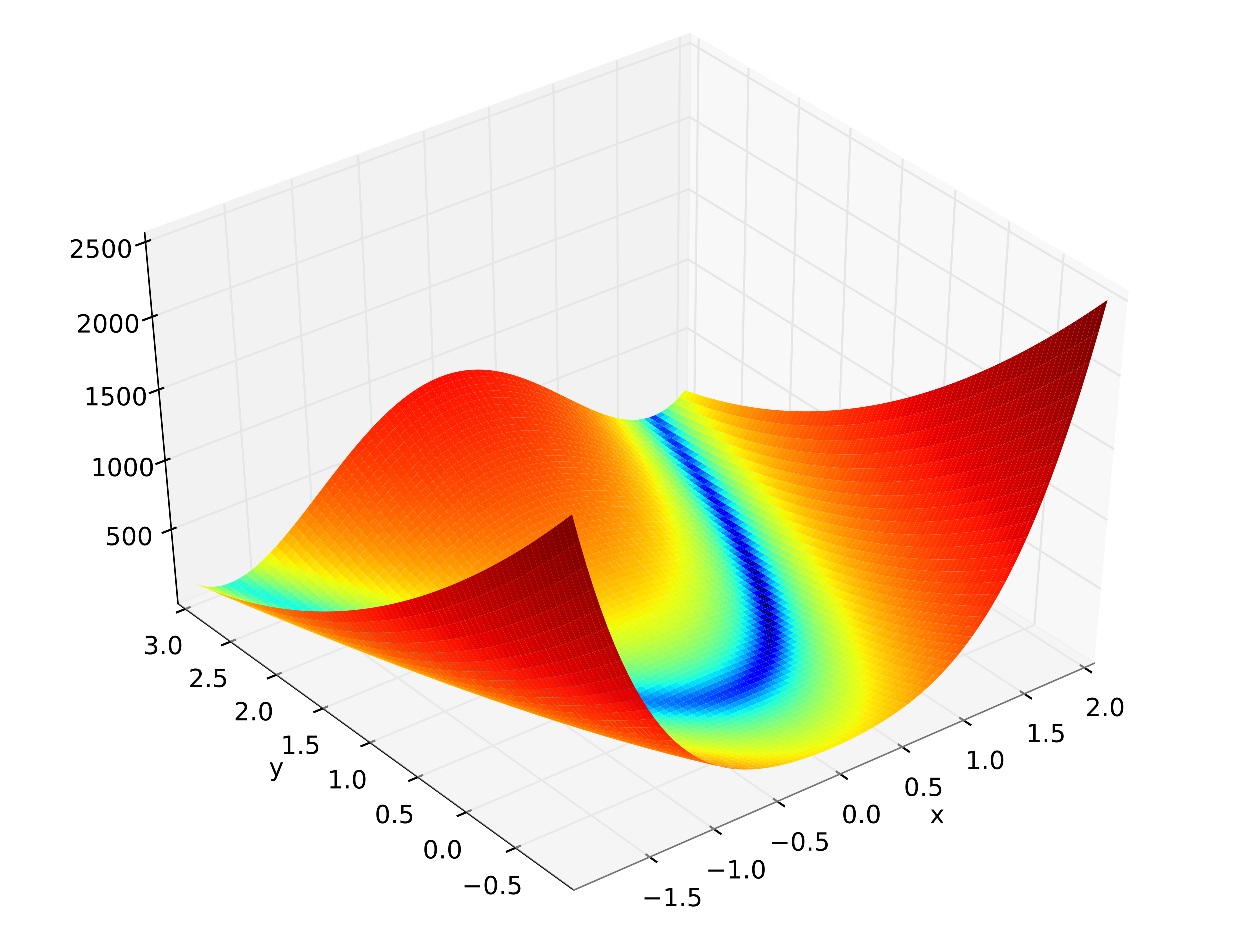
\includegraphics[width=.9\columnwidth]{rosenbrock}
        \end{center}
    \end{columns}
\end{frame}

\begin{frame}[fragile]
    \frametitle{StochasticSearch: Defining Search Spaces \& Tuning Runs}
    \alert{Parameters}:
    \begin{itemize}
        \item Represent \alert{individual optimizations}
        \item Determine \alert{ranges} and \alert{initial values}
        \item Integers, Booleans, Permutations, Strings, Enumerations, $\dots$
    \end{itemize}

    \pause

    Example:
    \begin{lstlisting}
FloatParameter(-2.0, 2.0, 0.0, "i0")
    \end{lstlisting}
\end{frame}

\begin{frame}[fragile]
    \frametitle{StochasticSearch: Defining Search Spaces \& Tuning Runs}
    \alert{Configurations}:
    \begin{itemize}
        \item Contain \alert{parameters}
        \item Describe the \alert{search space}
        \item Associate \alert{optimizations} with \alert{metrics}
    \end{itemize}

    \pause

    Example:
    \begin{lstlisting}
configuration = Configuration([FloatParameter(-2.0, 2.0, 0.0, "i0"),
                               FloatParameter(-2.0, 2.0, 0.0, "i1")],
                               "rosenbrock_config")
    \end{lstlisting}
\end{frame}

\begin{frame}[fragile]
    \frametitle{StochasticSearch: Defining Search Spaces \& Tuning Runs}
    \alert{Cost Function}:
    \begin{itemize}
        \item Computes \alert{costs} for each \alert{configuration}
        \item \alert{Costs} are usually expressed in \alert{floating point values}
    \end{itemize}

    \pause

    Example:
    \begin{lstlisting}
function rosenbrock(x::Configuration, parameters::Dict{Symbol, Any})
    return (1.0 - x["i0"].value)^2 + 100.0 * (x["i1"].value - x["i0"].value^2)^2
end
    \end{lstlisting}
\end{frame}

\begin{frame}[fragile]
    \frametitle{StochasticSearch: Defining Search Spaces \& Tuning Runs}
    \alert{Tuning Run}:
    \begin{itemize}
        \item Selection of \alert{search techniques}
        \item \alert{Duration} \& \alert{communication}
    \end{itemize}

    \pause

    Example:
    \begin{lstlisting}
tuning_run = Run(cost                = rosenbrock,
                 starting_point      = configuration,
                 stopping_criterion  = elapsed_time_criterion,
                 report_after        = 10,
                 reporting_criterion = elapsed_time_reporting_criterion,
                 duration            = 60,
                 methods             = [[:simulated_annealing 1];
                                        [:iterated_local_search 1];
                                        [:randomized_first_improvement 1];])
    \end{lstlisting}
\end{frame}

\begin{frame}
    \frametitle{StochasticSearch: More Examples}
    Short \alert{practical examples} at $\,$ \url{github.com/phrb/StochasticSearch.jl}:

    \begin{itemize}
        \item Rosenbrock
        \item Sorting Algorithm Cutoff
        \item Travelling Salesperson Problem
    \end{itemize}
\end{frame}

\section*{Next Steps}

\begin{frame}
    \frametitle{StochasticSearch: Next Steps}
    In \alert{future work}, we will:

    \begin{itemize}
        \item Run experiments with HPE's \alert{DPE simulators}
        \item Validate our approach on \alert{many-core and cloud scenarios}
        \item Develop strategies for \alert{expensive-to-evaluate cost functions}
    \end{itemize}
\end{frame}

\maketitle

\end{document}
